% Options for packages loaded elsewhere
\PassOptionsToPackage{unicode}{hyperref}
\PassOptionsToPackage{hyphens}{url}
%
\documentclass[
]{article}
\usepackage{amsmath,amssymb}
\usepackage{iftex}
\ifPDFTeX
  \usepackage[T1]{fontenc}
  \usepackage[utf8]{inputenc}
  \usepackage{textcomp} % provide euro and other symbols
\else % if luatex or xetex
  \usepackage{unicode-math} % this also loads fontspec
  \defaultfontfeatures{Scale=MatchLowercase}
  \defaultfontfeatures[\rmfamily]{Ligatures=TeX,Scale=1}
\fi
\usepackage{lmodern}
\ifPDFTeX\else
  % xetex/luatex font selection
\fi
% Use upquote if available, for straight quotes in verbatim environments
\IfFileExists{upquote.sty}{\usepackage{upquote}}{}
\IfFileExists{microtype.sty}{% use microtype if available
  \usepackage[]{microtype}
  \UseMicrotypeSet[protrusion]{basicmath} % disable protrusion for tt fonts
}{}
\makeatletter
\@ifundefined{KOMAClassName}{% if non-KOMA class
  \IfFileExists{parskip.sty}{%
    \usepackage{parskip}
  }{% else
    \setlength{\parindent}{0pt}
    \setlength{\parskip}{6pt plus 2pt minus 1pt}}
}{% if KOMA class
  \KOMAoptions{parskip=half}}
\makeatother
\usepackage{xcolor}
\usepackage[margin=1in]{geometry}
\usepackage{graphicx}
\makeatletter
\def\maxwidth{\ifdim\Gin@nat@width>\linewidth\linewidth\else\Gin@nat@width\fi}
\def\maxheight{\ifdim\Gin@nat@height>\textheight\textheight\else\Gin@nat@height\fi}
\makeatother
% Scale images if necessary, so that they will not overflow the page
% margins by default, and it is still possible to overwrite the defaults
% using explicit options in \includegraphics[width, height, ...]{}
\setkeys{Gin}{width=\maxwidth,height=\maxheight,keepaspectratio}
% Set default figure placement to htbp
\makeatletter
\def\fps@figure{htbp}
\makeatother
\setlength{\emergencystretch}{3em} % prevent overfull lines
\providecommand{\tightlist}{%
  \setlength{\itemsep}{0pt}\setlength{\parskip}{0pt}}
\setcounter{secnumdepth}{-\maxdimen} % remove section numbering
\newlength{\cslhangindent}
\setlength{\cslhangindent}{1.5em}
\newlength{\csllabelwidth}
\setlength{\csllabelwidth}{3em}
\newlength{\cslentryspacingunit} % times entry-spacing
\setlength{\cslentryspacingunit}{\parskip}
\newenvironment{CSLReferences}[2] % #1 hanging-ident, #2 entry spacing
 {% don't indent paragraphs
  \setlength{\parindent}{0pt}
  % turn on hanging indent if param 1 is 1
  \ifodd #1
  \let\oldpar\par
  \def\par{\hangindent=\cslhangindent\oldpar}
  \fi
  % set entry spacing
  \setlength{\parskip}{#2\cslentryspacingunit}
 }%
 {}
\usepackage{calc}
\newcommand{\CSLBlock}[1]{#1\hfill\break}
\newcommand{\CSLLeftMargin}[1]{\parbox[t]{\csllabelwidth}{#1}}
\newcommand{\CSLRightInline}[1]{\parbox[t]{\linewidth - \csllabelwidth}{#1}\break}
\newcommand{\CSLIndent}[1]{\hspace{\cslhangindent}#1}
\ifLuaTeX
  \usepackage{selnolig}  % disable illegal ligatures
\fi
\IfFileExists{bookmark.sty}{\usepackage{bookmark}}{\usepackage{hyperref}}
\IfFileExists{xurl.sty}{\usepackage{xurl}}{} % add URL line breaks if available
\urlstyle{same}
\hypersetup{
  pdftitle={Trauma treatment delay},
  pdfauthor={Anton Wasielewski},
  hidelinks,
  pdfcreator={LaTeX via pandoc}}

\title{Trauma treatment delay}
\usepackage{etoolbox}
\makeatletter
\providecommand{\subtitle}[1]{% add subtitle to \maketitle
  \apptocmd{\@title}{\par {\large #1 \par}}{}{}
}
\makeatother
\subtitle{A retrospective cohort study on the factors affecting the
delays in trauma care}
\author{Anton Wasielewski}
\date{}

\begin{document}
\maketitle

\hypertarget{introduction}{%
\section{Introduction}\label{introduction}}

\hypertarget{definition}{%
\subsection{Definition}\label{definition}}

Trauma, defined as the clinical entity composed of physical injury and
the body's associated response (1), is and has long been a major cause
of death around the world today (2). Within modern hospital care, the
trauma system stands as an important part in healthcare and is crucial
to lowering mortality and morbidity in injured patients through many
means, such as hospital care, follow up and prevention programs (3).

\hypertarget{trauma-statistics}{%
\subsection{Trauma Statistics}\label{trauma-statistics}}

Trauma is often divided into two subgroups, blunt force trauma and
penetrating trauma. Blunt force trauma is when an object or force
strikes the body, often causing bruising, broken bones or deep cuts.
Examples of blunt trauma could be car crashes, falls or direct blows to
the body. Penetrating trauma is when an object pierces the skin or body
and creates an open wound. Examples of penetrating trauma are gunshot
wounds and stab wounds (4). Differences exist between the two groups, as
blunt trauma patients tend to be more injured on arrival to the hospital
and as such, require more resources and are hospitalized for a longer
periods (5).

Today, trauma takes the lives of around 4,4 million people each year,
almost 8\% of all deaths (2). In the United States, trauma is the 4th
leading cause of death among the general population and the leading
cause for people between the ages of 1 and 44 (6). It is also an
important cause of hospitalization and morbidity among all age groups,
including seniors, and is responsible for an estimated 10\% of all years
lived with a disability globally. This has a significant burden on
social and economic level, costing countries billions of US dollars each
year in healthcare and lost productivity (7). Studies estimate the cost
of trauma care being between 18,500\$ and 41,500\$ per patient in high
income countries (HIC), depending on the country (8). However, it has
been shown that this burden is not evenly distributed between or within
countries. Many social factors such as age, sex and social status play a
major role in the risk of dying from trauma, with young men with low
socio-economic status being at most risk (2). But it is not only patient
level factors that affect what effect trauma has on people. About 90\%
of all trauma related deaths occur in low- and middle-income countries
(LMIC), with death rates by trauma also being higher than in high income
countries. Even within these LMIC, people of poorer socio-economic
status have higher death rates from trauma. Problems identified within
these countries that contribute to these statisitics were
infrastructure, education and training, attributed to lack of funding,
brain drain to HIC and lack of availability of basic amenities (9). In
HIC where funding and governance over the healthcare system is better
designed, functioning trauma systems and dedicated trauma centers exist
that have been shown to lower mortality but also improve functional
outcome in trauma patients (10).

\hypertarget{trauma-systems}{%
\subsection{Trauma systems}\label{trauma-systems}}

Trauma systems are infrastructures that exist to provide and optimize
care for injured patients starting with injury recognition and triage,
transport to appropriate trauma center, inpatient care and outpatient
follow-up. Beyond the clinical side, trauma systems work with outreach,
education and advocacy, data collection through registries, research,
funding, and disaster preparedness and response. A comprehensive and
functioning trauma system requires strong leadership and engagement at
the trauma center, regional and national level (7). This system is
crucial to provide care for trauma patients, both in reducing morbidity
and mortality in this patient group. Earlier studies from Sweden have
shown that treating severely injured patients at a trauma center is
associated with a 41\% lower adjusted 30-day mortality rate compared to
being treated at a non trauma care center due to them being more capable
of treating these patients, with potential survival benefit increasing
with higher injury severity (11). Other studies have shown similar
results, showing that treating injured patients at trauma centers is
associated with a 15-30\% decrease in mortality {[}(12); @Celso\_2006;
(13); @Haas\_2012{]} . During the last three decades, the introduction
of trauma systems has contributed to lowering the incidence of
preventable death . This is attributed to the improvements in care for
acute brain injuries and bleeding control. The incidence of late death
because of sepsis and multiple organ failure, possibly a result of
better and earlier resuscitation (14). Functioning trauma systems saves
lives in the hospital, but their work outside of the hospital is just as
important. Data collection from injured patients, such as mechanism of
injury or mortality, are essential for creating databases that can be
used for research. In turn, that research can be used for planning
injury prevention programs that target the most common injuries in the
right ways, e.g.~teen drivers, children, specific occupations etc. These
injury prevention programs can be planned on trauma center,
organizational or government level(15).

Trauma teams are multidisciplinary and operate in these centers. They
play a pivotal role in the treatment of the trauma patient, as they
provide the initial care in the critical stage of trauma. In Sweden,
trauma teams are lead by a team leader who is a surgeon, and include
practitioners from the specialities of intensive care, orthopedics,
nursing and support staff(16). For the trauma team to be mobilized,
trauma code has to be activated, often by an emergency nurse. The nurse
uses information gathered by the first responders to see if the patient
fits any of the criteria for trauma code. Most healthcare facilities
have established criteria or guidelines that trigger trauma code
activation. These criteria typically include mechanisms of injury,
physiological criteria, anatomical criteria and other specific
indicators of severe trauma. There are different levels of trauma code
with different criteria correlating with severity of injury, with level
1 mobilizing the most personnel to the trauma room. Once in the trauma
room, the team works systematically to manage the patients injuries.
They handle the most urgent problems first, such as airways and
breathing, with the aim to rapidly assess and stabilise the patient,
prioritise their injuries and arrange for site of definitive care. (17)

\hypertarget{mortality-and-morbidity-mom-conferences}{%
\subsection{Mortality and morbidity (MoM)
conferences}\label{mortality-and-morbidity-mom-conferences}}

Many hospitals have a trauma registry where they log the patients
information and timeline of what happened. The extent of the registry
varies, with HIC having more complete registries. This logging of
information is important work, as a cornerstone of trauma quality
improvement programs is multidisciplinary MoM conferences. The MoM
conference is a meeting where different specialities who work with
trauma care sit down and discuss deaths and complications in order to
look for preventable factors. These conferences are performed in many
hospitals globally, almost everywhere where there are formal medical
specialty departments and sometimes in smaller hospitals as well (18).
In Sweden, many hospitals have mortality conferences on deceased patient
cases, but only one has MoM conferences to better their trauma care on
patients who lived (19). The reason being that this expansion of MoM
conferences takes time and resources, which is why all hospitals don't
implement this.

The endpoint of these MoM conferences are opportunities for improvement
(OFI). At the end of the conference, consensus is reached regarding the
existence of an OFI and implementation of corrective action. This
process is effective, as it has been shown that this review is
associated with high-quality trauma care (20). Examples of OFI may
include lack of resources and management errors. One common OFI is
delayed treatment. According to previous studies, among the preventable
or possibly preventable deaths in trauma patients, delay in treatment
has been identified as a major error contributing to death, found in up
to 52.9\% of patients in said group (21). Delayed treatment has been
shown to have adverse effects on patients, showing why it is such an
important issue and the need to develop strategies to combat {[}(22);
@Sampalis\_1994{]}. Although it is such a common OFI, the patient level
factors associated with delayed treatment are poorly understood. There
may be several factors that correlate with receiving delayed treatment,
but they have yet to be identified. Mapping these factors may help in
identifying patients that might be at risk for receiving delayed
treatment before it happens.

\hypertarget{aim}{%
\subsection{Aim}\label{aim}}

The aim of this paper is to determine what different patient level
factors affect the risk of receiving delayed treatment at a trauma
center.

\hypertarget{methods}{%
\section{Methods}\label{methods}}

\hypertarget{setting}{%
\subsection{Setting}\label{setting}}

Every year, Karolinska University hospital, which is the equivalent of a
trauma level 1 hospital, admits 1500 trauma patients each year. To be
added to the trauma registry, a patient must be over 15 years of age,
had ISS\textgreater9 and/or had trauma code activation. They get added
to both the Karolinska Trauma registry as well as the national trauma
registry (SweTrau). The registry includes data on vital signs, injuries,
interventions and patient information. Another database, the trauma care
quality database includes information relevant for MoM conferences. At
Karolinska University Hospital, patients who die during hospital stay
gets their case sent to a MoM everytime. However, for the rest of the
patients, two specialized nurses determine whether they are. Several
audit filters are set up to flag for patients with possible OFIs.
Flagged patients are then reviewed by these two nurses who decide if
there is a possible OFI, in which case their case is sent to a MoM
conference for further review.

\hypertarget{study-design}{%
\subsection{Study design}\label{study-design}}

We conducted a registry based cohort study using data from the trauma
registry and trauma care quality database at the Karolinska University
Hospital in Solna. The trauma registry includes about 14000 patients
treated between 2012 and 2022. The trauma care quality database is a
subset of the trauma registry and includes about 8000 patients selected
for review between 2013 and 2022. This project will link the two
databases and assess how different patient level factors, such as age,
sex, mechanism of injury, and injury severity, are associated with
delayed treatment using logistic regression.

\hypertarget{outcome}{%
\subsection{Outcome}\label{outcome}}

The outcome is delayed treatment, as identified by the multidisciplinary
review board and recorded in the trauma care quality database.

\hypertarget{participants}{%
\subsection{Participants}\label{participants}}

The database only includes patients 15 years old and above, ISS
\textgreater9 and/or trauma team activation. Inclusion in the study
further requires that the patients have been assessed for OFIs. Patients
were excluded if they were missing information in one of the examined
patient factors.

\hypertarget{variables}{%
\subsection{Variables}\label{variables}}

The outcome is delayed treatment, which is defined as more than 30
minutes passing from arrival before receiving treatment, as identified
by the multidisciplinary review board and recorded in the trauma care
quality database.

\hypertarget{data-sourcesmeasurement}{%
\subsection{Data sources/measurement}\label{data-sourcesmeasurement}}

The data comes from the trauma registry and trauma care quality
database.

\hypertarget{bias}{%
\subsection{Bias}\label{bias}}

Selection bias as this is a retrospective cohort study where the outcome
has occurred.

Misclassification bias as the conference may reach a consensus that is
wrong.

\hypertarget{study-size}{%
\subsection{Study size}\label{study-size}}

The study size is all of the eligible patients that was treated at the
hospital between 2012 and 2022. Starting 2013 only a subgroup of
patients were screened for OFIs, but starting 2017 all patients that are
included in the database are screened for OFIs.

\hypertarget{statistical-methods}{%
\subsection{Statistical methods}\label{statistical-methods}}

Multivariable and potentially univariable logistical regression. A 5\%
significance level and 95\% confidence levels will be used.

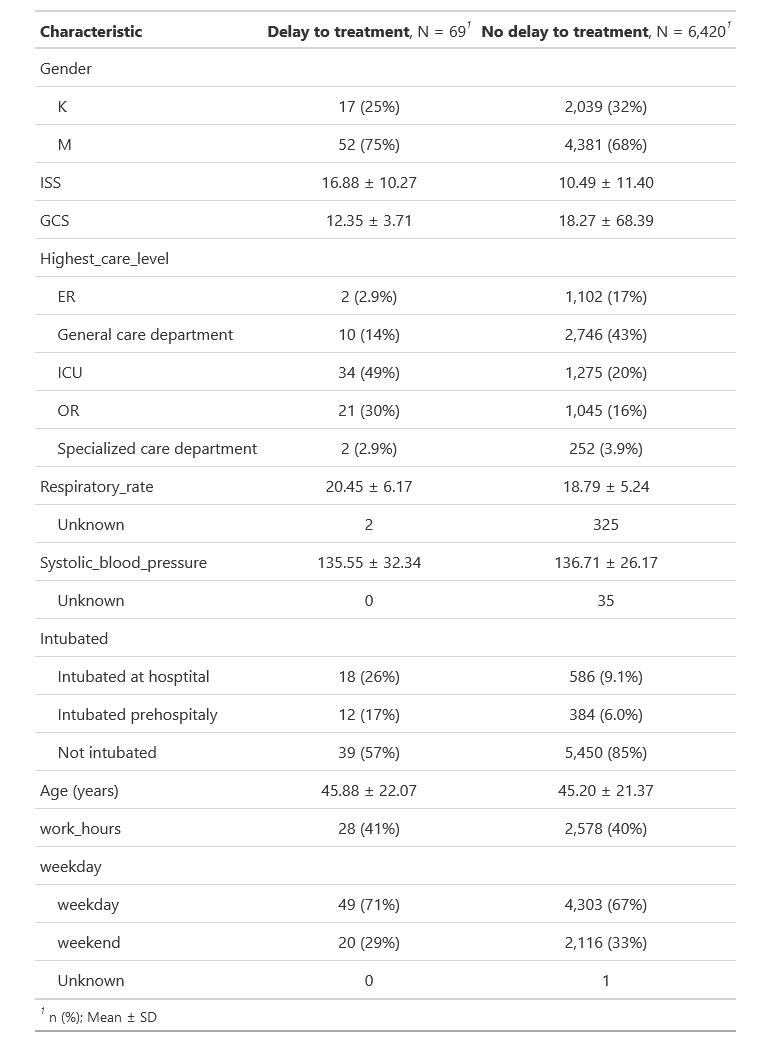
\includegraphics{table1.html}

\hypertarget{ethical-considerations}{%
\subsection*{Ethical considerations}\label{ethical-considerations}}
\addcontentsline{toc}{subsection}{Ethical considerations}

\hypertarget{refs}{}
\begin{CSLReferences}{0}{0}
\leavevmode\vadjust pre{\hypertarget{ref-gerdin_risk_2015}{}}%
\CSLLeftMargin{1. }%
\CSLRightInline{Gerdin M. The risk of dying: Predicting trauma mortality
in urban indian hospitals. Stockholm: Karolinska Institutet; 2015. }

\leavevmode\vadjust pre{\hypertarget{ref-WHO_2021}{}}%
\CSLLeftMargin{2. }%
\CSLRightInline{Injuries and violence {[}Internet{]}. World Health
Organization. World Health Organization; 2021. Available from:
\url{https://www.who.int/news-room/fact-sheets/detail/injuries-and-violence}}

\leavevmode\vadjust pre{\hypertarget{ref-Choi_2021}{}}%
\CSLLeftMargin{3. }%
\CSLRightInline{Choi J, Carlos G, Nassar AK, Knowlton LM, Spain DA. The
impact of trauma systems on patient outcomes {[}Internet{]}. Current
problems in surgery. U.S. National Library of Medicine; 2021. Available
from: \url{https://www.ncbi.nlm.nih.gov/pmc/articles/PMC7286246/}}

\leavevmode\vadjust pre{\hypertarget{ref-NIGMS_2020}{}}%
\CSLLeftMargin{4. }%
\CSLRightInline{General Medical Sciences NI of. Physical trauma
{[}Internet{]}. National Institute of General Medical Sciences. U.S.
Department of Health; Human Services; 2020. Available from:
\url{https://nigms.nih.gov/education/fact-sheets/Pages/physical-trauma.aspx}}

\leavevmode\vadjust pre{\hypertarget{ref-FITCH2019}{}}%
\CSLLeftMargin{5. }%
\CSLRightInline{Blunt versus penetrating trauma: Is there a resource
intensity discrepancy? The American Journal of Surgery {[}Internet{]}.
2019;218(6):1201--5. Available from:
\url{https://www.sciencedirect.com/science/article/pii/S0002961019303861}}

\leavevmode\vadjust pre{\hypertarget{ref-AAST_2020}{}}%
\CSLLeftMargin{6. }%
\CSLRightInline{AAST. Trauma\_facts\_and\_links {[}Internet{]}. The
American Association for the Surgery of Trauma. The American Association
for the Surgery of Trauma; 2020. Available from:
\url{https://www.aast.org/resources/trauma-facts}}

\leavevmode\vadjust pre{\hypertarget{ref-connolly_2018}{}}%
\CSLLeftMargin{7. }%
\CSLRightInline{Connolly R, Woo MY, Lampron J, Perry JJ.
\href{https://doi.org/10.1017/cem.2017.389}{Factors associated with
delay in trauma team activation and impact on patient outcomes}.
Canadian Journal of Emergency Medicine. 2018;20(4):606--13. }

\leavevmode\vadjust pre{\hypertarget{ref-Willenberg_2012}{}}%
\CSLLeftMargin{8. }%
\CSLRightInline{Willenberg L, Curtis K, Taylor C, Jan S, Glass P,
Myburgh J. \href{https://doi.org/10.1186/1472-6963-12-267}{The variation
of acute treatment costs of trauma in high-income countries}. BMC Health
Services Research. 2012;12(1). }

\leavevmode\vadjust pre{\hypertarget{ref-Shanthakumar_2021}{}}%
\CSLLeftMargin{9. }%
\CSLRightInline{Shanthakumar D, Payne A, Leitch T, Alfa-Wali M.
\href{https://doi.org/10.1055/s-0041-1732351}{Trauma care in low- and
middle-income countries}. The Surgery Journal. 2021;07(04). }

\leavevmode\vadjust pre{\hypertarget{ref-Nirula_2006}{}}%
\CSLLeftMargin{10. }%
\CSLRightInline{Nirula R, Brasel K.
\href{https://doi.org/10.1097/01.ta.0000230305.36456.4e}{Do trauma
centers improve functional outcomes: A national trauma databank
analysis?} The Journal of Trauma: Injury, Infection, and Critical Care.
2006 Aug;61(2):268--71. }

\leavevmode\vadjust pre{\hypertarget{ref-Candefjord_2020}{}}%
\CSLLeftMargin{11. }%
\CSLRightInline{Candefjord S, Asker L, Caragounis E-C.
\href{https://doi.org/10.1007/s00068-020-01446-6}{Mortality of trauma
patients treated at trauma centers compared to non-trauma centers in
sweden: A retrospective study}. European Journal of Trauma and Emergency
Surgery. 2020;48(1):525--36. }

\leavevmode\vadjust pre{\hypertarget{ref-Moran_2018}{}}%
\CSLLeftMargin{12. }%
\CSLRightInline{Moran CG, Lecky F, Bouamra O, Lawrence T, Edwards A,
Woodford M, et al.
\href{https://doi.org/10.1016/j.eclinm.2018.07.001}{Changing the system
- major trauma patients and their outcomes in the NHS (england)
2008--17}. EClinicalMedicine. 2018;2--3:13--21. }

\leavevmode\vadjust pre{\hypertarget{ref-MacKenzie_2006}{}}%
\CSLLeftMargin{13. }%
\CSLRightInline{MacKenzie EJ, Rivara FP, Jurkovich GJ, Nathens AB, Frey
KP, Egleston BL, et al. \href{https://doi.org/10.1056/nejmsa052049}{A
national evaluation of the effect of trauma-center care on mortality}.
New England Journal of Medicine. 2006;354(4):366--78. }

\leavevmode\vadjust pre{\hypertarget{ref-Asensio_2008}{}}%
\CSLLeftMargin{14. }%
\CSLRightInline{Asensio J, Trunkey D. Current therapy of trauma and
surgical critical care. Elsevier; 2008. }

\leavevmode\vadjust pre{\hypertarget{ref-ACS}{}}%
\CSLLeftMargin{15. }%
\CSLRightInline{ACS. Trauma systems consultation program {[}Internet{]}.
ACS. Available from:
\url{https://www.facs.org/quality-programs/trauma/systems/trauma-systems-consultation-program/}}

\leavevmode\vadjust pre{\hypertarget{ref-vuxe4stra_G}{}}%
\CSLLeftMargin{16. }%
\CSLRightInline{Johnsson E. Traumateamet -- roller och ansvar
{[}Internet{]}. 2020. Available from:
\url{https://mellanarkiv-offentlig.vgregion.se/alfresco/s/archive/stream/public/v1/source/available/sofia/hs9766-305841775-25/surrogate/Traumateamet\%20-\%20roller\%20och\%20ansvar.pdf}}

\leavevmode\vadjust pre{\hypertarget{ref-Hedberg_2020}{}}%
\CSLLeftMargin{17. }%
\CSLRightInline{Hedberg M, Falkén M, Wihlke G, Jansson S, Hultgren J,
Eriksson S, et al. Traumamanual {[}Internet{]}.
Traumamanual\_Karolinska\_Universitetssjukhuset\_Solna. NKS; 2020.
Available from:
\url{https://traumarummet.files.wordpress.com/2020/09/traumamanualen-2020.pdf}}

\leavevmode\vadjust pre{\hypertarget{ref-WHO_2009}{}}%
\CSLLeftMargin{18. }%
\CSLRightInline{Guidelines for trauma quality improvement programmes
{[}Internet{]}. World Health Organization. World Health Organization;
2009. Available from:
\url{https://www.who.int/publications/i/item/guidelines-for-trauma-quality-improvement-programmes}}

\leavevmode\vadjust pre{\hypertarget{ref-SweTrau_2023}{}}%
\CSLLeftMargin{19. }%
\CSLRightInline{SweTrau. Täckningsgrad {[}Internet{]}. Täckningsgrad
\textbar{} SweTrau. 2023. Available from:
\url{https://rcsyd.se/swetrau/om-swetrau/tackningsgrad}}

\leavevmode\vadjust pre{\hypertarget{ref-Santana_2014}{}}%
\CSLLeftMargin{20. }%
\CSLRightInline{Santana MJ, Stelfox HT.
\href{https://doi.org/10.1097/sla.0b013e31828df98e}{Development and
evaluation of evidence-informed quality indicators for adult injury
care}. Annals of Surgery. 2014;259(1):186--92. }

\leavevmode\vadjust pre{\hypertarget{ref-Teixeira_2007}{}}%
\CSLLeftMargin{21. }%
\CSLRightInline{Teixeira PG, Inaba K, Hadjizacharia P, Brown C, Salim A,
Rhee P, et al.
\href{https://doi.org/10.1097/ta.0b013e31815078ae}{Preventable or
potentially preventable mortality at a mature trauma center}. Journal of
Trauma: Injury, Infection \&amp;amp; Critical Care. 2007
Dec;63(6):1338--47. }

\leavevmode\vadjust pre{\hypertarget{ref-Sampalis_1995}{}}%
\CSLLeftMargin{22. }%
\CSLRightInline{Sampalis JS, Boukas S, Lavoie A, Nikolis A, Frechette P,
Brown R, et al.
\href{https://doi.org/10.1097/00005373-199512000-00002}{Preventable
death evaluation of the appropriateness of the on-site trauma care
provided by urgences-sante physicians}. The Journal of Trauma: Injury,
Infection, and Critical Care. 1995;39(6):1029--35. }

\end{CSLReferences}

\end{document}
